\subsection{Conversion Manager [Simone]}
\label{sec:Insieme.Frontend.Convert}

\begin{figure}[tb]
	\centering
	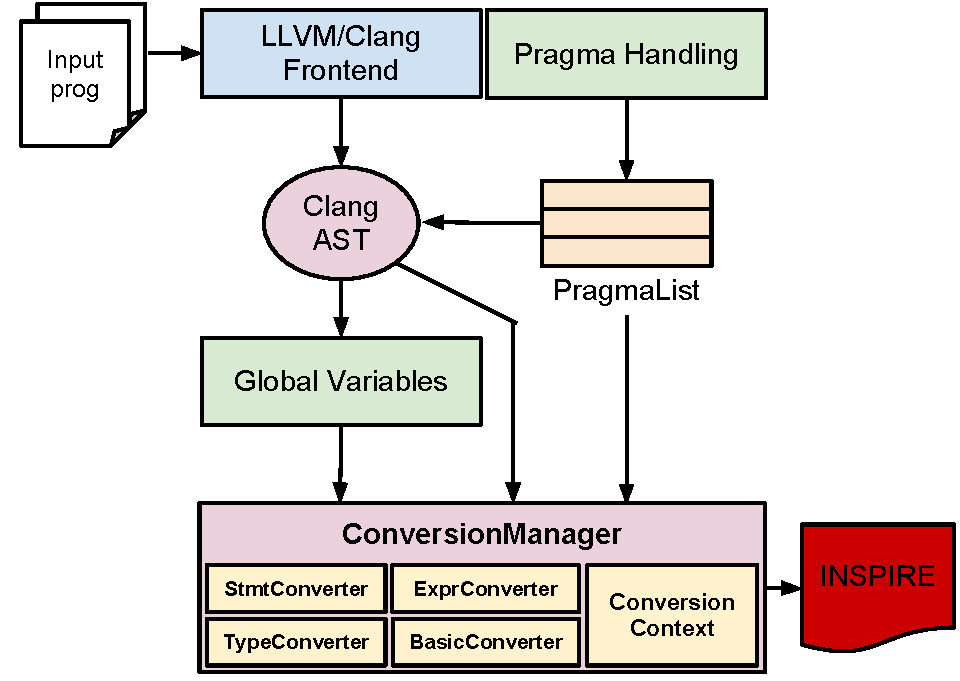
\includegraphics[width=0.8\textwidth]{compiler/frontend/seq_frontend.pdf}
	\caption{Dataflow of the Insieme Frontend}
	\label{fig:Frontend.Seq}
\end{figure}

In Figure~\ref{fig:Frontend.Seq}, the flow of execution of the frontend is
depicted. We already explained two component which are executed before the
actual conversion into IR is performed. The task of converting the {\tt
LLVM/Clang} AST is done by the \type{frontend::Conversion\-Manager}. In order
to reduce the complexity of the conversion procedure, we split the code into 4
"converters" taking care of specific aspects of the C language:

\begin{description}

\item [BasicConverter:] Defined in \file{frontend/basic\_convert.cpp}. It
contains utility functions which are used across all the converters.

\item [TypeConvert:]  Defined in \file{frontend/type\_convert.cpp}. It takes care
of the conversion of C/C++ types into IR types. 

\item [StmtConverter:] Defined in \file{frontend/stmt\_convert.cpp}. It takes care
of the conversion of C/C++ statements into IR statements. 

\item[ExprConverter:] Defined in \file{frontend/expr\_convert.cpp}. It takes care
of the conversion of C/C++ expressions into IR statements. 

\end{description}

To make the code readable, the implementation of the 4 converters are spread
across 4 translation units. Also, because of optimization issues related to the
amount of symbols being exported by the frontend {\tt .so} library, the
definition of those converters is completely hidden and not accessible outside
the frontend.  Because the \type{frontend::Con\-ver\-sion\-Manager} provides a facade
for invoking the conversion facility, so there is no need for external access of
the single converters. Communication among converters is obtained through the
manager class, this means that each converter can utilize functionalities of
another converter (or himself) through the \type{frontend::ConversionManager}
class whose interface is defined in \file{frontend/convert.h}.
Indeed the manager class provides 3 fundamental methods: 

\begin{description}
\item [{\tt TypePtr convertType(const clang::Type*)}:] Converts an {\tt
LLVM/Clang} type node into an INSIPRE type.

\item [{\tt ExpressionPtr convertExpr(const clang::Expr*)}:] Converts an
{\tt LLVM/Clang} expression node into an INSPIRE expression. 

\item [{\tt StatementPtr convertStmt(const clang::Stmt*)}:] Converts an
{\tt LLVM/Clang} statement node into an INSPIRE statement.

\end{description}

Beside taking care of dispatching the conversion task to the appropriate
converter, the manager also performs some optimizations at this stage in order
to speedup the conversion process. For example, by introducing caching we avoid
to convert symbols which have already been converted. Caching is not utilized
for all types of IR nodes as the probability of converting two identical
statements is very low. However, caching is quite successful for types nodes as
the type reference to type node ration is high. Future PhDs might be interested
in speeding up the frontend time and introducing smarter way of caching nodes
could be a simple and high effective way of doing it (low hanging fruit).

Finally, the manager also retains a context which stores information necessary
through the conversion process of the IR. In the context we store those
information which needs to be visible (or alive) during the conversion of the
entire program. For example, the mapping between a Clang variable declaration
and an IR variable makes sure the same C variable is being replaced by the same IR
entity consistently for all the encountered references to it. 

\subsubsection{Type Converter}
{\tt LLVM/Clang} supports a visitor interface for traversing the AST. For this
reason the class \type{frontend::TypeConverter} inherits from
\type{clang::TypeVisitor}. The visitor defines several methods which define how
the C AST node should be transformed into IR. Each method of the visitor returns
the generated node so that the IR representation of complex node can be built
upon composition of the type node returned by successive calls to the visitor
itself. 

One peculiarity of the \type{frontend::TypeConverter} is the way we deal with
pointers type. Indeed, the IR type system doesn't support the C semantics of
pointers which not necessary refers to the element directly pointed in memory.
For example, in C a pointer can be used to refer to an array of elements or a
singular scalar variables. Ideally the
following conversion semantics shall be used for pointer:

\begin{table}
\begin{centering}
	\begin{tabular}{l|c}
		\textbf{C Type} & \textbf{IR Type} \\
		\hline \hline
		\constant{type* (R-Value)}          & \insCodeInl{ref<'type>} \\
		\constant{type* (L-Value)} 		   & \insCodeInl{ref<ref<'type>} \\
		\hline 
	\end{tabular}
	\caption{Sound type conversions for C pointers}
	\label{tab:Compiler.Frontend.ml.GenNNoutput}
\end{centering}
\end{table}

However, because we must take into account situation for which the pointer is
used to refer to an array, and the user want to access a memory location which
is not at displacement 0, then a different encoding is necessary in order to
guarantee sound semantics check of the generated IR program. For these reason
the following encoding is utilized: 

\begin{table}
\begin{centering}
	\begin{tabular}{l|c}
		\textbf{C Type} & \textbf{IR Type} \\
		\hline \hline
		\constant{type* (R-Value)}          & \insCodeInl{ref<array<'type,1>>} \\
		\constant{type* (L-Value)} 		   & \insCodeInl{ref<ref<array<'type,1>>>} \\
		\hline 
	\end{tabular}
	\caption{Implemented type conversions for C pointers}
	\label{tab:Compiler.Frontend.ml.GenNNoutput}
\end{centering}
\end{table}

\note{Proposal for 'array-erasure' procedure useful to cleanup
generated IR.}
This however introduces several levels of ugliness to the IR code being
generated by the frontend. One way to really deal with this problem is to apply
a two phase approach which shall be implemented in Insieme. Because we don't
want to perform any advanced analysis on the input code, we let the frontend
produce an IR code which contains impurities (for example representing pointers
using IR arrays as it is now). Right after the frontend completes the
conversion, we may apply an analysis (on the generated IR) which data mine the
type of usage of pointers. If for example a pointer is always used to access the
element at displacement 0 then we can safely replace the IR type to be a
\insCodeInl{ref<'type>}. Those situations where the pointer is being used to
access elements with an offset not equal zero, then the array type should be
maintained. In those cases, DEF-USE \todo{ref DEF-USE} analysis may be used to
determine the declaration of the array being addressed and if possible replace
the \insCodeInl{ref<array<'type>>} with an actual
\insCodeInl{ref<vector<'type,N>>}. All of these are options which may be
implemented right after the first phase of the frontend has been processed. It
may improve both the readability of the generated IR code and possibility for
optimizations. 

Most type conversion is straightforward, the only exception are {\tt struct}
types which may cause a problem due to the possibility to have cyclic
references. As discussed in the overview, an IR node cannot be build if the
children are not already available, therefore trying to building a node
referring to himself is not possible. The same type of problem happens for
recursive function calls and this is handled in the IR using special recursive
types and lambda definitions which will be covered
in~\ref{sec:Insieme.Frontend.Recursion}. 

\subsubsection{Statement Converter}

Conversion of statements is done in a similar way types are converted. Each
statement generates an equivalent IR statement. However it can happen that one
\type{clang::Stmt} node can generate multiple INSPIRE statements. This is the
case of declaration statements for example where one declaration statement can
declare several variables. In INSPIRE this is not allowed as, for simplicity, a
declaration statement only declare a single variable. Therefore, differently
from the type conversion, the output of a visit method of the
\type{frontend::StmtVisitor} is of type \type{frontend::StmtWrapper} which is-a
vector of statements. It is worth noting that we couldn't do any different since
by wrapping multiple statements into a compound statements for example would
have yield to different program semantics (e.g. declared variables must be
visible by following statements in the same scope). In order to simplify the
handling of the return value of the visitor methods we defined the {\tt
tryToAggregateStmts()} function which takes care of wrapping (when necessary)
the returned list of statements into one statement (by embedding them into a
compound statement). 

Most conversion of C statements are straightforward, however some of them
require some special kind of analysis in order for the conversion to be
performed. An example are loop statements. In C loop statements have a much more
complex definition than the INSPIRE for loop. For example, in C is possible to
use a for statement to implement the semantics of a while loop (using an empty
initialization statement and a boolean exit condition). Or otherwise, multiple
induction variables can be defined for a for-statement and this is also not
allowed in INSPIRE where a loop statement only contains one induction variable.
In order to determine whether a C loop statement can be represented using the
INSPIRE for statement we perform an analysis. This is implemented in the
\file{frontend/include/insieme/frontend/analysis/loop\_analyzer.h}. The
\type{frontend::analysis::LoopAnalyzer} class tries to retrieve three important
piece of information from a given for statement. 

\begin{description}
\item [Induction Variable:] The first thing is to determine the induction
variable of the for loop, this is done by extracting the set of  variables
defined in the initialization section of the for statement and intersect it with
the variable being used in the loop condition and increment operation. If the
result of the intersection is one variable, then this variable is selected to be
the induction variable for this loop. In the contrary case, an exception is
thrown in the constructor of the \type{LoopAnalyzer} class containing a message
which explains the reason why this statement cannot be represented as an IR for
statement. 

\item[Exit Condition:] Because in the IR the specification for a for loop is
based on the upper bound of the induction variable, the condition expression of a
C for statement needs to be manipulated in order to isolate the upper bound.
This is what the result of the {\tt LoopAnalyzer::getCondExpr()} method is. 

\item[Increment Expression:] The last piece of information is the value of the
increment step which is also extracted from the C definition of the for
statement. 

\end{description}

If the analyzer managers to extract without any ambiguities those pieces of
information, then the actual conversion of the for statement begins. Otherwise
an exception will be launched, of type
\type{frontend::analysis::LoopNormalizationError}, and the frontend will create
a while statement which is semantically equivalent to the for statement.  

Another big difference between C for statements and the INSPIRE for statement is
the fact the INSPIRE for always declare the induction variable and it cannot use
an existing variable for that. In such cases the frontend takes care of
introducing a new induction variable, initialize its value and at the exit point
of the for statement make sure that correct value is assigned to the original
induction variable. Details on the implementation are available in the
source code. 

Another aspect where the INSPIRE code differs from C semantics is the switch
statement. Indeed while in C the switch statement has a fall-through semantics
(which means the switch will execute the code contained in all cases following
the entry point case, unless {\tt break} is utilized), in INSPIRE there is no
such a thing. Therefore each case contains statements which are executed when
that branch is taken. This requires to copy several time the list of statement
in the case the original switch statement was written using the fall-through
semantics. 

\subsubsection{Expression Converter}



